\documentclass{article}
\twocolumn
\usepackage[utf8]{inputenc}
\usepackage{geometry}
\usepackage{amsmath}
\usepackage{amsthm}
\usepackage{mathtools}
\usepackage{commath}
\usepackage{tikz}
\usepackage{listings}
\usepackage{graphicx}
\graphicspath{ {./images/} }

\title{\textbf{\Huge Assignment 1}}
\author{\large H.N Srikanth - SM21Mtech12012}

\date{August 2021}

\begin{document}

\providecommand{\mbf}{\mathbf}

\newcommand{\myvec}[1]{\ensuremath{\begin{pmatrix}#1\end{pmatrix}}}
\let\vec\mathbf

\maketitle

\section*{Chapter II, Examples II}
\textbf{Q22 (iii)}
\textbf{Find the conditions that the four points}

\myvec{x_1\\y_1}, \myvec{x_2\\y_2},
\myvec{x_3\\y_3}, \myvec{x_4\\y_4}

\textbf{ may be the vertices of a rhombus.}\\

\textbf{Solution :}

The given points are
\begin{align*}
\begin{split}
\vec{A} = \myvec{x_1\\y_1}, \vec{B} =\myvec{x_2\\y_2},\\
\vec{C} =\myvec{x_3\\y_3}, \vec{D} =\myvec{x_4\\y_4},\\
\end{split}
\end{align*}
Conditions for the given four points to be the vertices of a rhombus are:
\begin{enumerate}
  \item If opposite sides are parallel and
  \item If diagonals are perpendicular .
\end{enumerate}
if

\begin{equation}\label{first_equation}
(\vec{A}-\vec{B} ) = k(\vec{D}-\vec{C} )
\end{equation}
\begin{equation}\label{second_equation}
(\vec{B}-\vec{C} )=k(\vec{A}-\vec{D} )
\end{equation}

{here k is any integer.}
\eqref{first_equation} shows 
$$AB \parallel DC $$
\eqref{second_equation} shows 
$$BC \parallel AD$$

if 
\begin{equation}\label{Third_equation}
(\vec{A}-\vec{C} )^ \top ( \vec{B}-\vec{D} ) = 0 
\end{equation}

\eqref{Third_equation} shows
$$AC \perp BD $$
{As the given four points satisfy the required conditions we can say that they are the vertices of a rhombus.}\\
\textbf{Numerical Example :}
 
{Examine whether the given points A (2,-3) and B (6,5) and C (-2,1) and D (-6,-7) forms a rhombus.}\\

 \textbf{Sol:}
 The given points are
\begin{align} 
\vec{A} = \myvec{2\\-3},\vec{B} =\myvec{6\\5},\\
\vec{C} =\myvec{-2\\1}, \vec{D} =\myvec{-6\\-7}\\
(\vec{A}-\vec{B} ) = \myvec{-4\\-8}, (\vec{D}-\vec{C} ) = \myvec{-4\\-8}\\
(\vec{B}-\vec{C} ) = \myvec{8\\4}, (\vec{A}-\vec{D} ) = \myvec{8\\4}
\end{align} 

\begin{equation}\label{Eight_equation}
(\vec{A}-\vec{B} ) = (\vec{D}-\vec{C} )  \\
\end{equation}
\begin{equation}\label{Ninth_equation}
(\vec{B}-\vec{C} )  = (\vec{A}-\vec{D} ) 
\end{equation}

{As k=1 in \eqref{Eight_equation} and \eqref{Ninth_equation}}

\eqref{Eight_equation} shows $$ AB  {\parallel} DC $$ and \eqref{Ninth_equation} shows $$BC \parallel AD $$\\
    
\begin{align}
(\vec{A}-\vec{C} )^\top = \myvec{4&-4 }
,(\vec{B}-\vec{D} ) = \myvec{12\\12}
\end{align}
\begin{equation}\label{Eleventh_equation}
(\vec{A}-\vec{C} )^ \top ( \vec{B}-\vec{D} ) = 48-48 = 0
\end{equation}
 \eqref{Eleventh_equation} shows
$$AC \perp BD $$\\ 
{Given points A,B,C,D satisfy the required 
conditions hence they form a Rhombus.}

{Rhombus is drawn using python}
\begin{lstlisting}
https://github.com/Srikanth1408/Assignment_1/blob/main/Assignment1.ipynb
\end{lstlisting}
\begin{figure}[!ht]
	\centering
	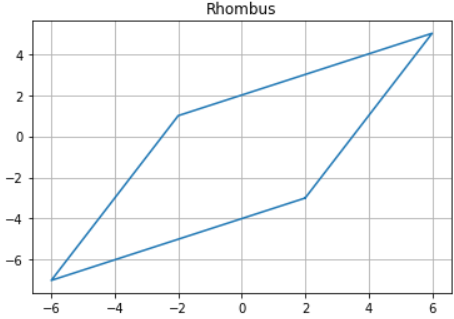
\includegraphics[width=\columnwidth]{rhombus.png}
	\caption{The given points form a rhombus}
\end{figure}
\end{document}